\chaptersub{Symmetric Modes}{Private Key Cryptography}

\section{Block Ciphers}
    A \textbf{block cipher} is type of encryption based on \textbf{permutation}, where they key, $\{0,1\}^k$, defines a transposition of bits in the block to the encrypted, $\{0,1\}^b$. The block is a proportion of the message.\\
    \\
    DES was the first civilian block cipher and was developed at IBM in the 1970s. When the US government adopted it, they recommended the following four ways to use it, these are now used with any block cipher.
    \begin{itemize}
        \item Electronic Code Book
        \item Cipher Block Chaining
        \item Counter
        \item ...
    \end{itemize}
    
    \subsection{Electronic Code Book}
    This is a very simple, it \textbf{divides} the message into blocks of size $b$, pads the last one, and \textbf{encrypts them all individually}. A block cipher using ECB is only OW-CPA, as Figure~\ref{fig:ecb-attacktable} says. This the terrible!\\
    \begin{figure}[htp!]
    \centering
    \attacktable{owcpa}
    \caption{Security Models ECB passes}
    \label{fig:ecb-attacktable}
    \end{figure}
    \\
    The weakness of this mode is in the fact that the blocks of encrypted independently. This is the basis for the two attacks below, but it also means it's susceptible to \textbf{block replay}. That is where an adversary edits a bit knowing how it will affect the decrypted message. If I knew you were sending me some money, and I knew the block containing the amount you were transferring, I could change that block in the hope I would end up with a larger transaction. This could be fixed with a checksum. ECB has one positive that an error in the cipher text will not propagate to other blocks when decrypted.\\
    \\
    \textbf{Proving a cryptographic system passes a security model is beyond this scope of this course}, but you should be able to give an intuitive reason. It passes OW-CPA because, with only an encryption oracle, you would have to brute-force every possible message to match it with the ciphertext. We can always make $b$ large enough so that this is not possible.\footnote{This might be possible if you knew the context of the message, if you understand what is being sent and the domain of possible values of a block is relatively small. This is simply poor implementation of the encryption, however, and we don't worry about that.}\\
    \\
    \textbf{OW-CCA Example:} We can win an OW-CCA game by kind of cheating in the following way. If we have a decryption oracle, we can decrypt anything that is not the message. Since the blocks are independent, we can simply split the message in half and decrypt both individually and then concatenate the result.\\
    \\
    \textbf{IND-PASS Example:} In an Indistinguishability game we decide the message (of which one will be encrypted). Again we use the fact that the blocks are encrypted independently, and give one of the message as a bit string concatenated onto itself, $m_0=b_1||b_1$. The ciphertext can be split into two equal bit strings in the same way, then it was that message.
    
    
    
    \subsection{Cipher Block Chaining}
    Cipher Block Chaining removes a lot of the problems with the ECB by XORing each block with the previously encrypted block --- incorporating a dependence on the previous block. The first block of the ciphertext is called the \textbf{Initalisation Vector} (IV), and is what the first block of the message is XOR-ed with.\\
    \begin{figure}[htp!]
        \centering
        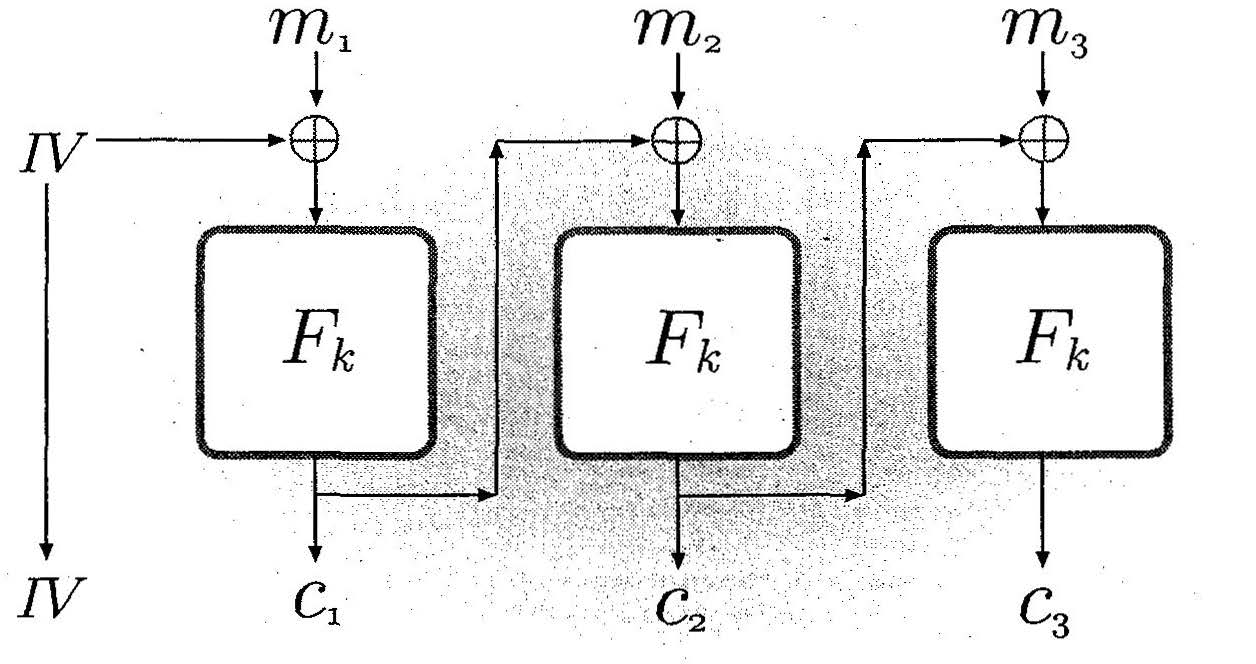
\includegraphics[width=10cm]{img/cbc}
        \caption{Diagram of CBC encrypting}
    \end{figure}
    \\
    More formally:\nopagebreak
    \begin{center}
    \begin{tabular}{lll}
    \textbf{Encryption}:                                        && \textbf{Decryption}\\
    $c_0 = IV$                                                  && $IV = c_0$\\
    $c_1 = Enc_k(m_1 \oplus IV)$                                && $m_1 = Dec_k(c_1) \oplus IV$\\
    $c_i = Enc_k(m_i \oplus c_{i-1}) \textrm{ for } i > 1$      && $m_i = Dec_k(c_i) \oplus c_{i-1} \textrm{ for } i > 1$\\
    \end{tabular}
    \end{center}
    \begin{figure}[htp!]
        \centering
        \attacktable{indcpa}
        \caption{Security of Models CBC}
        \label{fig:cbc-attacktable}
    \end{figure}
    Note that $IV$ is sent unencrypted, because it is needed for decryption. This can seem pointless, but if it is generated randomly every time, then it means that encryption is probabilistic. CBC is OW-CPA and IND-CPA but not OW-CCA or IND-CCA.\\
    \begin{figure}[htp!]
        \centering
        \begin{subfigure}[b]{0.3\textwidth}
            \centering
            
\includegraphics[width=\textwidth]{img/Tux.jpg}
            \caption{Original Image\\~}
        \end{subfigure}
        \begin{subfigure}[b]{0.3\textwidth}
            \centering
            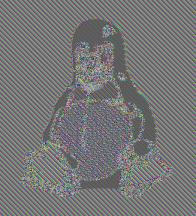
\includegraphics[width=\textwidth]{img/Tux_ecb.jpg}
            \caption{Encrypted using ECB\\~}
        \end{subfigure}
        \begin{subfigure}[b]{0.3\textwidth}
            \centering
            
\includegraphics[width=\textwidth]{img/Tux_secure.jpg}
            \caption{Encrypted using Chaining}
        \end{subfigure}
        \caption{Bitmap image of Tux being encrypted using ECB and using another method that uses chaining.}
        \label{fig:tux}
    \end{figure}
    \\
    \textbf{With a decryption oracle, CBC will fail} because of the same trick used before --- we can ask to oracle to decrypt the ciphertext with extra blocks on the end.
    
    
    
    \subsection{Counter Mode}
    Counter mode is the same as CBC mode, but 

\section{Message Authentication}
    \subsection{Why Do This}
        Encrypting data provides confidentiality (remember the three goals), but does not provide authenticity or integrity without additional sauce. This is the additional sauce.
        It comes with two flavours that are used for different things: \textbf{MDC} (Manipulation Detection Codes) and \textbf{MAC} (Message Authentication Codes). We will worry about \textbf{MAC}


    \subsection{\textbf{M}essage \textbf{A}uthentication \textbf{C}odes}
    MAC codes are the result of hashing the message, using a hash function that takes a key.
    \begin{figure}[htp!]
        \centering
        MAC = $h_{k}(m)$
    \end{figure}